% Options for packages loaded elsewhere
\PassOptionsToPackage{unicode}{hyperref}
\PassOptionsToPackage{hyphens}{url}
%
\documentclass[
  ignorenonframetext,
  aspectratio=169,
]{beamer}
\usepackage{pgfpages}
\setbeamertemplate{caption}[numbered]
\setbeamertemplate{caption label separator}{: }
\setbeamercolor{caption name}{fg=normal text.fg}
\beamertemplatenavigationsymbolsempty
% Prevent slide breaks in the middle of a paragraph
\widowpenalties 1 10000
\raggedbottom
\setbeamertemplate{part page}{
  \centering
  \begin{beamercolorbox}[sep=16pt,center]{part title}
    \usebeamerfont{part title}\insertpart\par
  \end{beamercolorbox}
}
\setbeamertemplate{section page}{
  \centering
  \begin{beamercolorbox}[sep=12pt,center]{part title}
    \usebeamerfont{section title}\insertsection\par
  \end{beamercolorbox}
}
\setbeamertemplate{subsection page}{
  \centering
  \begin{beamercolorbox}[sep=8pt,center]{part title}
    \usebeamerfont{subsection title}\insertsubsection\par
  \end{beamercolorbox}
}
\AtBeginPart{
  \frame{\partpage}
}
\AtBeginSection{
  \ifbibliography
  \else
    \frame{\sectionpage}
  \fi
}
\AtBeginSubsection{
  \frame{\subsectionpage}
}
\usepackage{amsmath,amssymb}
\usepackage{lmodern}
\usepackage{iftex}
\ifPDFTeX
  \usepackage[T1]{fontenc}
  \usepackage[utf8]{inputenc}
  \usepackage{textcomp} % provide euro and other symbols
\else % if luatex or xetex
  \usepackage{unicode-math}
  \defaultfontfeatures{Scale=MatchLowercase}
  \defaultfontfeatures[\rmfamily]{Ligatures=TeX,Scale=1}
\fi
\usetheme[]{metropolis}
\usecolortheme{seahorse}
% Use upquote if available, for straight quotes in verbatim environments
\IfFileExists{upquote.sty}{\usepackage{upquote}}{}
\IfFileExists{microtype.sty}{% use microtype if available
  \usepackage[]{microtype}
  \UseMicrotypeSet[protrusion]{basicmath} % disable protrusion for tt fonts
}{}
\makeatletter
\@ifundefined{KOMAClassName}{% if non-KOMA class
  \IfFileExists{parskip.sty}{%
    \usepackage{parskip}
  }{% else
    \setlength{\parindent}{0pt}
    \setlength{\parskip}{6pt plus 2pt minus 1pt}}
}{% if KOMA class
  \KOMAoptions{parskip=half}}
\makeatother
\usepackage{xcolor}
\IfFileExists{xurl.sty}{\usepackage{xurl}}{} % add URL line breaks if available
\IfFileExists{bookmark.sty}{\usepackage{bookmark}}{\usepackage{hyperref}}
\hypersetup{
  pdftitle={Session 1},
  pdfauthor={Matt Denwood and Eleftherios Meletis},
  hidelinks,
  pdfcreator={LaTeX via pandoc}}
\urlstyle{same} % disable monospaced font for URLs
\newif\ifbibliography
\usepackage{color}
\usepackage{fancyvrb}
\newcommand{\VerbBar}{|}
\newcommand{\VERB}{\Verb[commandchars=\\\{\}]}
\DefineVerbatimEnvironment{Highlighting}{Verbatim}{commandchars=\\\{\}}
% Add ',fontsize=\small' for more characters per line
\usepackage{framed}
\definecolor{shadecolor}{RGB}{248,248,248}
\newenvironment{Shaded}{\begin{snugshade}}{\end{snugshade}}
\newcommand{\AlertTok}[1]{\textcolor[rgb]{0.94,0.16,0.16}{#1}}
\newcommand{\AnnotationTok}[1]{\textcolor[rgb]{0.56,0.35,0.01}{\textbf{\textit{#1}}}}
\newcommand{\AttributeTok}[1]{\textcolor[rgb]{0.77,0.63,0.00}{#1}}
\newcommand{\BaseNTok}[1]{\textcolor[rgb]{0.00,0.00,0.81}{#1}}
\newcommand{\BuiltInTok}[1]{#1}
\newcommand{\CharTok}[1]{\textcolor[rgb]{0.31,0.60,0.02}{#1}}
\newcommand{\CommentTok}[1]{\textcolor[rgb]{0.56,0.35,0.01}{\textit{#1}}}
\newcommand{\CommentVarTok}[1]{\textcolor[rgb]{0.56,0.35,0.01}{\textbf{\textit{#1}}}}
\newcommand{\ConstantTok}[1]{\textcolor[rgb]{0.00,0.00,0.00}{#1}}
\newcommand{\ControlFlowTok}[1]{\textcolor[rgb]{0.13,0.29,0.53}{\textbf{#1}}}
\newcommand{\DataTypeTok}[1]{\textcolor[rgb]{0.13,0.29,0.53}{#1}}
\newcommand{\DecValTok}[1]{\textcolor[rgb]{0.00,0.00,0.81}{#1}}
\newcommand{\DocumentationTok}[1]{\textcolor[rgb]{0.56,0.35,0.01}{\textbf{\textit{#1}}}}
\newcommand{\ErrorTok}[1]{\textcolor[rgb]{0.64,0.00,0.00}{\textbf{#1}}}
\newcommand{\ExtensionTok}[1]{#1}
\newcommand{\FloatTok}[1]{\textcolor[rgb]{0.00,0.00,0.81}{#1}}
\newcommand{\FunctionTok}[1]{\textcolor[rgb]{0.00,0.00,0.00}{#1}}
\newcommand{\ImportTok}[1]{#1}
\newcommand{\InformationTok}[1]{\textcolor[rgb]{0.56,0.35,0.01}{\textbf{\textit{#1}}}}
\newcommand{\KeywordTok}[1]{\textcolor[rgb]{0.13,0.29,0.53}{\textbf{#1}}}
\newcommand{\NormalTok}[1]{#1}
\newcommand{\OperatorTok}[1]{\textcolor[rgb]{0.81,0.36,0.00}{\textbf{#1}}}
\newcommand{\OtherTok}[1]{\textcolor[rgb]{0.56,0.35,0.01}{#1}}
\newcommand{\PreprocessorTok}[1]{\textcolor[rgb]{0.56,0.35,0.01}{\textit{#1}}}
\newcommand{\RegionMarkerTok}[1]{#1}
\newcommand{\SpecialCharTok}[1]{\textcolor[rgb]{0.00,0.00,0.00}{#1}}
\newcommand{\SpecialStringTok}[1]{\textcolor[rgb]{0.31,0.60,0.02}{#1}}
\newcommand{\StringTok}[1]{\textcolor[rgb]{0.31,0.60,0.02}{#1}}
\newcommand{\VariableTok}[1]{\textcolor[rgb]{0.00,0.00,0.00}{#1}}
\newcommand{\VerbatimStringTok}[1]{\textcolor[rgb]{0.31,0.60,0.02}{#1}}
\newcommand{\WarningTok}[1]{\textcolor[rgb]{0.56,0.35,0.01}{\textbf{\textit{#1}}}}
\usepackage{graphicx}
\makeatletter
\def\maxwidth{\ifdim\Gin@nat@width>\linewidth\linewidth\else\Gin@nat@width\fi}
\def\maxheight{\ifdim\Gin@nat@height>\textheight\textheight\else\Gin@nat@height\fi}
\makeatother
% Scale images if necessary, so that they will not overflow the page
% margins by default, and it is still possible to overwrite the defaults
% using explicit options in \includegraphics[width, height, ...]{}
\setkeys{Gin}{width=\maxwidth,height=\maxheight,keepaspectratio}
% Set default figure placement to htbp
\makeatletter
\def\fps@figure{htbp}
\makeatother
\setlength{\emergencystretch}{3em} % prevent overfull lines
\providecommand{\tightlist}{%
  \setlength{\itemsep}{0pt}\setlength{\parskip}{0pt}}
\setcounter{secnumdepth}{-\maxdimen} % remove section numbering
\makeatletter
\def\verbatim@nolig@list{}
\makeatother


% fontspec requires xelatex which gives problems for me (Matt)
% \usepackage{fontspec}
% % \setmainfont[Ligatures=Historic]{TeX Gyre Pagella}
% \newfontfamily\FiraCode{Fira Code}
% \setmonofont[Contextuals={Alternate}]{Fira Code}
% \newfontfamily\Fontify[Path = ../common/]{Fontify-Regular}
% \else
% \newcommand{\Fontify}{}
% \fi



% \usepackage{fontspec}
% \setmonofont{FiraCode-Regular}[Contextuals=Alternate]
% \usepackage{listings}
% \usepackage[verbatim]{lstfiracode}
% \lstset{style=FiraCodeStyle,basicstyle=\ttfamily}
\usepackage{xspace}
\newcommand{\rlang}[0]{\texttt{R}\xspace}

\newcommand{\rpackage}[1]{\texttt{\{#1\}}}
\newcommand{\dataset}[1]{\textsl{#1}}
% \newcommand{\hotkey}[1]{#1}

% this package is conflicted with the keystroke package.
% \usepackage{statex2}

\usepackage{keystroke}
\usepackage{fvextra}
\fvset{samepage=true}
\fvset{breaklines=true}
\fvset{baselinestretch=1}
%% Adds line numbers to R code chunks in beamer:
% \fvset{numbers=left}
\RecustomVerbatimEnvironment{verbatim}{Verbatim}{breaklines}
%% Controls the font size of R code chunks, but overrides any local settings:
% \fvset{fontsize=\scriptsize}
\usepackage{ccfonts}
\makeatletter
\beamer@ignorenonframefalse
\makeatother

\usepackage{comment}

\ifLuaTeX
  \usepackage{selnolig}  % disable illegal ligatures
\fi

\title{Session 1}
\subtitle{An introduction to JAGS}
\author{Matt Denwood and Eleftherios Meletis}
\date{2023-06-07}

\begin{document}
\frame{\titlepage}

\hypertarget{background}{%
\section{Background}\label{background}}

\begin{frame}[fragile]{Diagnostic test evaluation: with gold standard =
simple!}
\protect\hypertarget{diagnostic-test-evaluation-with-gold-standard-simple}{}
\scriptsize

\begin{Shaded}
\begin{Highlighting}[]
\FunctionTok{library}\NormalTok{(}\StringTok{"tidyverse"}\NormalTok{)}
\NormalTok{se }\OtherTok{\textless{}{-}} \FunctionTok{c}\NormalTok{(}\DecValTok{1}\NormalTok{, }\FloatTok{0.6}\NormalTok{)}
\NormalTok{sp }\OtherTok{\textless{}{-}} \FunctionTok{c}\NormalTok{(}\DecValTok{1}\NormalTok{, }\FloatTok{0.9}\NormalTok{)}
\NormalTok{N }\OtherTok{\textless{}{-}} \DecValTok{1000}
\NormalTok{prevalence }\OtherTok{\textless{}{-}} \FloatTok{0.25}

\NormalTok{data }\OtherTok{\textless{}{-}} \FunctionTok{tibble}\NormalTok{(}\AttributeTok{Status =} \FunctionTok{rbinom}\NormalTok{(N, }\DecValTok{1}\NormalTok{, prevalence)) }\SpecialCharTok{\%\textgreater{}\%}
  \FunctionTok{mutate}\NormalTok{(}\AttributeTok{Test1 =} \FunctionTok{rbinom}\NormalTok{(N, }\DecValTok{1}\NormalTok{, se[}\DecValTok{1}\NormalTok{]}\SpecialCharTok{*}\NormalTok{Status }\SpecialCharTok{+}\NormalTok{ (}\DecValTok{1}\SpecialCharTok{{-}}\NormalTok{sp[}\DecValTok{1}\NormalTok{])}\SpecialCharTok{*}\NormalTok{(}\DecValTok{1}\SpecialCharTok{{-}}\NormalTok{Status))) }\SpecialCharTok{\%\textgreater{}\%}
  \CommentTok{\# Which is the same as:}
  \FunctionTok{mutate}\NormalTok{(}\AttributeTok{Test1 =}\NormalTok{ Status) }\SpecialCharTok{\%\textgreater{}\%}
  \FunctionTok{mutate}\NormalTok{(}\AttributeTok{Test2 =} \FunctionTok{rbinom}\NormalTok{(N, }\DecValTok{1}\NormalTok{, se[}\DecValTok{2}\NormalTok{]}\SpecialCharTok{*}\NormalTok{Status }\SpecialCharTok{+}\NormalTok{ (}\DecValTok{1}\SpecialCharTok{{-}}\NormalTok{sp[}\DecValTok{2}\NormalTok{])}\SpecialCharTok{*}\NormalTok{(}\DecValTok{1}\SpecialCharTok{{-}}\NormalTok{Status)))}

\NormalTok{(twoXtwo }\OtherTok{\textless{}{-}} \FunctionTok{with}\NormalTok{(data, }\FunctionTok{table}\NormalTok{(Status, Test2)))}
\DocumentationTok{\#\#       Test2}
\DocumentationTok{\#\# Status   0   1}
\DocumentationTok{\#\#      0 656  68}
\DocumentationTok{\#\#      1 127 149}
\end{Highlighting}
\end{Shaded}

\normalsize

\pause

\scriptsize

\begin{Shaded}
\begin{Highlighting}[]
\NormalTok{(sensitivity }\OtherTok{\textless{}{-}}\NormalTok{ twoXtwo[}\DecValTok{2}\NormalTok{,}\DecValTok{2}\NormalTok{] }\SpecialCharTok{/} \FunctionTok{sum}\NormalTok{(twoXtwo[}\DecValTok{2}\NormalTok{,}\DecValTok{1}\SpecialCharTok{:}\DecValTok{2}\NormalTok{]))}
\DocumentationTok{\#\# [1] 0.5398551}
\NormalTok{(specificity }\OtherTok{\textless{}{-}}\NormalTok{ twoXtwo[}\DecValTok{1}\NormalTok{,}\DecValTok{1}\NormalTok{] }\SpecialCharTok{/} \FunctionTok{sum}\NormalTok{(twoXtwo[}\DecValTok{1}\NormalTok{,}\DecValTok{1}\SpecialCharTok{:}\DecValTok{2}\NormalTok{]))}
\DocumentationTok{\#\# [1] 0.9060773}
\end{Highlighting}
\end{Shaded}

\normalsize
\end{frame}

\begin{frame}[fragile]{Diagnostic test evaluation: no gold standard}
\protect\hypertarget{diagnostic-test-evaluation-no-gold-standard}{}
Now we have both values of sensitivity and specificity
\textless1\ldots{}

\scriptsize

\begin{Shaded}
\begin{Highlighting}[]
\NormalTok{se }\OtherTok{\textless{}{-}} \FunctionTok{c}\NormalTok{(}\FloatTok{0.9}\NormalTok{, }\FloatTok{0.6}\NormalTok{)}
\NormalTok{sp }\OtherTok{\textless{}{-}} \FunctionTok{c}\NormalTok{(}\FloatTok{0.95}\NormalTok{, }\FloatTok{0.9}\NormalTok{)}
\NormalTok{N }\OtherTok{\textless{}{-}} \DecValTok{1000}
\NormalTok{prevalence }\OtherTok{\textless{}{-}} \FloatTok{0.25}

\NormalTok{data }\OtherTok{\textless{}{-}} \FunctionTok{tibble}\NormalTok{(}\AttributeTok{Status =} \FunctionTok{rbinom}\NormalTok{(N, }\DecValTok{1}\NormalTok{, prevalence)) }\SpecialCharTok{\%\textgreater{}\%}
  \FunctionTok{mutate}\NormalTok{(}\AttributeTok{Test1 =} \FunctionTok{rbinom}\NormalTok{(N, }\DecValTok{1}\NormalTok{, se[}\DecValTok{1}\NormalTok{]}\SpecialCharTok{*}\NormalTok{Status }\SpecialCharTok{+}\NormalTok{ (}\DecValTok{1}\SpecialCharTok{{-}}\NormalTok{sp[}\DecValTok{1}\NormalTok{])}\SpecialCharTok{*}\NormalTok{(}\DecValTok{1}\SpecialCharTok{{-}}\NormalTok{Status))) }\SpecialCharTok{\%\textgreater{}\%}
  \FunctionTok{mutate}\NormalTok{(}\AttributeTok{Test2 =} \FunctionTok{rbinom}\NormalTok{(N, }\DecValTok{1}\NormalTok{, se[}\DecValTok{2}\NormalTok{]}\SpecialCharTok{*}\NormalTok{Status }\SpecialCharTok{+}\NormalTok{ (}\DecValTok{1}\SpecialCharTok{{-}}\NormalTok{sp[}\DecValTok{2}\NormalTok{])}\SpecialCharTok{*}\NormalTok{(}\DecValTok{1}\SpecialCharTok{{-}}\NormalTok{Status)))}

\FunctionTok{with}\NormalTok{(data, }\FunctionTok{table}\NormalTok{(Status, Test1))}
\DocumentationTok{\#\#       Test1}
\DocumentationTok{\#\# Status   0   1}
\DocumentationTok{\#\#      0 691  35}
\DocumentationTok{\#\#      1  32 242}
\FunctionTok{with}\NormalTok{(data, }\FunctionTok{table}\NormalTok{(Status, Test2))}
\DocumentationTok{\#\#       Test2}
\DocumentationTok{\#\# Status   0   1}
\DocumentationTok{\#\#      0 667  59}
\DocumentationTok{\#\#      1 104 170}
\end{Highlighting}
\end{Shaded}

\normalsize
\end{frame}

\begin{frame}[fragile]
In real life we don't know what \texttt{Status} is\ldots{}

\scriptsize

\begin{Shaded}
\begin{Highlighting}[]
\NormalTok{(twoXtwo }\OtherTok{\textless{}{-}} \FunctionTok{with}\NormalTok{(data, }\FunctionTok{table}\NormalTok{(Test1, Test2)))}
\DocumentationTok{\#\#      Test2}
\DocumentationTok{\#\# Test1   0   1}
\DocumentationTok{\#\#     0 646  77}
\DocumentationTok{\#\#     1 125 152}
\NormalTok{(sensitivity\_1 }\OtherTok{\textless{}{-}}\NormalTok{ twoXtwo[}\DecValTok{2}\NormalTok{,}\DecValTok{2}\NormalTok{] }\SpecialCharTok{/} \FunctionTok{sum}\NormalTok{(twoXtwo[}\DecValTok{1}\SpecialCharTok{:}\DecValTok{2}\NormalTok{,}\DecValTok{2}\NormalTok{]))}
\DocumentationTok{\#\# [1] 0.6637555}
\NormalTok{(sensitivity\_2 }\OtherTok{\textless{}{-}}\NormalTok{ twoXtwo[}\DecValTok{2}\NormalTok{,}\DecValTok{2}\NormalTok{] }\SpecialCharTok{/} \FunctionTok{sum}\NormalTok{(twoXtwo[}\DecValTok{2}\NormalTok{,}\DecValTok{1}\SpecialCharTok{:}\DecValTok{2}\NormalTok{]))}
\DocumentationTok{\#\# [1] 0.5487365}
\NormalTok{(specificity\_1 }\OtherTok{\textless{}{-}}\NormalTok{ twoXtwo[}\DecValTok{1}\NormalTok{,}\DecValTok{1}\NormalTok{] }\SpecialCharTok{/} \FunctionTok{sum}\NormalTok{(twoXtwo[}\DecValTok{1}\SpecialCharTok{:}\DecValTok{2}\NormalTok{,}\DecValTok{1}\NormalTok{]))}
\DocumentationTok{\#\# [1] 0.8378729}
\NormalTok{(specificity\_2 }\OtherTok{\textless{}{-}}\NormalTok{ twoXtwo[}\DecValTok{1}\NormalTok{,}\DecValTok{1}\NormalTok{] }\SpecialCharTok{/} \FunctionTok{sum}\NormalTok{(twoXtwo[}\DecValTok{1}\NormalTok{,}\DecValTok{1}\SpecialCharTok{:}\DecValTok{2}\NormalTok{]))}
\DocumentationTok{\#\# [1] 0.8934993}
\end{Highlighting}
\end{Shaded}

\normalsize

\pause

So we will \emph{always} under-estimate the Se and Sp of both tests!
\end{frame}

\begin{frame}[fragile]{The solution}
\protect\hypertarget{the-solution}{}
\begin{itemize}
\item
  We need to assess the sensitivity and specificity of both tests
  against the true (but unknown) \texttt{Status} of each individual
\item
  This unknown \texttt{Status} is called the \texttt{latent\ class}

  \begin{itemize}
  \tightlist
  \item
    Therefore we need to run a \texttt{latent\ class\ model} \ldots{}
  \end{itemize}
\end{itemize}

\pause

\begin{itemize}
\tightlist
\item
  How can we implement a latent class model?

  \begin{itemize}
  \tightlist
  \item
    Frequentist statistical methods:

    \begin{itemize}
    \tightlist
    \item
      possible, but difficult
    \end{itemize}
  \item
    Bayesian statistical methods:

    \begin{itemize}
    \tightlist
    \item
      easier and much more commonly done!
    \end{itemize}
  \end{itemize}
\end{itemize}
\end{frame}

\begin{frame}[fragile]{Learning outcomes}
\protect\hypertarget{learning-outcomes}{}
By the end of the course you should be able to:

\begin{itemize}
\item
  Understand what a latent class model is, and how they can be used for
  diagnostic test evaluation
\item
  Run basic latent class models using R and JAGS for real-world problems
\item
  Interpret the results
\item
  Understand the nuances and complexities associated with these types of
  analysis and the interpretation of the \texttt{latent\ class}
\end{itemize}
\end{frame}

\hypertarget{revision}{%
\section{Revision}\label{revision}}

\begin{frame}{Bayes Rule}
\protect\hypertarget{bayes-rule}{}
Bayes' theorem is at the heart of Bayesian statistics:

\[P(\theta|Y) = \frac{P(\theta)\times P(Y|\theta)}{P(Y)}\]

\pause

Where: \(\theta\) is our parameter value(s);

\(Y\) is the data that we have observed;

\(P(\theta|Y)\) is the posterior probability of the parameter value(s);

\(P(\theta)\) is the prior probability of the parameters;

\(P(Y|\theta)\) is the likelihood of the data given the parameters
value(s);

\(P(Y)\) is the probability of the data, integrated over parameter
space.
\end{frame}

\begin{frame}
\begin{itemize}
\tightlist
\item
  In practice we usually work with the following:
\end{itemize}

\[P(\theta|Y) \propto P(\theta)\times P(Y|\theta)\]

\pause

\begin{itemize}
\item
  Our Bayesian posterior is therefore always a combination of the
  likelihood of the data, and the parameter priors
\item
  But for more complex models the distinction between what is `data' and
  `parameters' can get blurred!
\end{itemize}
\end{frame}

\begin{frame}{MCMC}
\protect\hypertarget{mcmc}{}
\begin{itemize}
\item
  A way of obtaining a numerical approximation of the posterior
\item
  Highly flexible
\item
  Not inherently Bayesian but most widely used in this context
\item
  Assessing convergence is essential, otherwise we may not be
  summarising the true posterior
\item
  Our chains are correlated so we need to consider the effective sample
  size
\end{itemize}
\end{frame}

\begin{frame}{Bayesian MCMC vs Frequentist ML}
\protect\hypertarget{bayesian-mcmc-vs-frequentist-ml}{}
Advantages:

\begin{itemize}
\tightlist
\item
  Very flexible modelling framework
\item
  More natural interpretation of confidence intervals (credible
  intervals)
\item
  Ability to incorporate prior information
\end{itemize}

\pause

Disadvantages:

\begin{itemize}
\tightlist
\item
  More computationally intensive
\item
  More emphasis on the practictioner to ensure the output is reliable
\item
  Requirement to incorporate prior information
\end{itemize}
\end{frame}

\begin{frame}{Everyone up to speed?}
\protect\hypertarget{everyone-up-to-speed}{}
Any questions so far?

Anything unclear?
\end{frame}

\begin{frame}{Practical points}
\protect\hypertarget{practical-points}{}
Each session has 2 versions:

\begin{itemize}
\item
  .html = the main file for you guys (includes exercises + solutions,
  code is copy/pasteable)
\item
  .pdf = presentation (probably best to ignore this as the html has the
  same content)
\end{itemize}

\pause

Other files (e.g.~data) required for a specific session will be in the
same folders as the .html files

\pause

You should completely ignore the ignore\_this\_folder folders!!
\end{frame}

\hypertarget{session-1-a-practical-introduction-to-mcmc}{%
\section{Session 1: A practical introduction to
MCMC}\label{session-1-a-practical-introduction-to-mcmc}}

\begin{frame}{MCMC in Practice}
\protect\hypertarget{mcmc-in-practice}{}
\begin{itemize}
\item
  We can write a Metropolis algorithm ourselves, but this is complex and
  inefficient
\item
  There are a number of general purpose languages that allow us to
  define the problem and leave the details to the software:

  \begin{itemize}
  \tightlist
  \item
    WinBUGS/OpenBUGS

    \begin{itemize}
    \tightlist
    \item
      Bayesian inference Using Gibbs Sampling
    \end{itemize}
  \item
    JAGS

    \begin{itemize}
    \tightlist
    \item
      Just another Gibbs Sampler
    \end{itemize}
  \item
    Stan

    \begin{itemize}
    \tightlist
    \item
      Named in honour of Stanislaw Ulam, pioneer of the Monte Carlo
      method
    \end{itemize}
  \end{itemize}
\end{itemize}
\end{frame}

\begin{frame}{JAGS}
\protect\hypertarget{jags}{}
\begin{itemize}
\item
  JAGS uses the BUGS language

  \begin{itemize}
  \tightlist
  \item
    This is a declarative (non-procedural) language
  \item
    The order of statements does not matter
  \item
    The compiler converts our model syntax into an MCMC algorithm with
    appropriately defined likelihood and prior
  \item
    You can only define each variable once!!!
  \end{itemize}
\end{itemize}

\pause

\begin{itemize}
\item
  Different ways to run JAGS from R:

  \begin{itemize}
  \tightlist
  \item
    rjags, runjags, R2jags, jagsUI
  \end{itemize}
\item
  See \url{http://runjags.sourceforge.net/quickjags.html}

  \begin{itemize}
  \tightlist
  \item
    This is also in the GitHub folder
  \end{itemize}
\end{itemize}
\end{frame}

\begin{frame}[fragile]
A simple JAGS model might look like this:

\scriptsize

\begin{verbatim}
model{
  # Likelihood part:
  Positives ~ dbinom(prevalence, N)
  
  # Prior part:
  prevalence ~ dbeta(1, 1)
  
  # Hooks for automatic integration with R:
  #data# Positives, N
  #monitor# prevalence
  #inits# prevalence
}
\end{verbatim}

\normalsize
\end{frame}

\begin{frame}[fragile]
There are two model statements:

\begin{itemize}
\tightlist
\item
  The first: \scriptsize
\end{itemize}

\begin{Shaded}
\begin{Highlighting}[]
\NormalTok{Positives }\SpecialCharTok{\textasciitilde{}} \FunctionTok{dbinom}\NormalTok{(prevalence, N)}
\end{Highlighting}
\end{Shaded}

\normalsize

states that the number of \texttt{Positive} test samples is Binomially
distributed with probability parameter \texttt{prevalence} and total
trials \texttt{N}

\pause

\begin{itemize}
\tightlist
\item
  The second: \scriptsize
\end{itemize}

\begin{Shaded}
\begin{Highlighting}[]
\NormalTok{prevalence }\SpecialCharTok{\textasciitilde{}} \FunctionTok{dbeta}\NormalTok{(}\DecValTok{1}\NormalTok{,}\DecValTok{1}\NormalTok{)}
\end{Highlighting}
\end{Shaded}

\normalsize

states that our prior probability distribution for the parameter
\texttt{prevalence} is Beta(1,1), which is the same as Uniform(0,1)

\pause

These are very similar to the likelihood and prior functions defined in
the preparatory exercise (although this prior is less informative)
\end{frame}

\begin{frame}[fragile]
The other lines in this model:

\scriptsize

\begin{Shaded}
\begin{Highlighting}[]
\CommentTok{\#data\# Positives, N}
\CommentTok{\#monitor\# prevalence}
\CommentTok{\#inits\# prevalence}
\end{Highlighting}
\end{Shaded}

\normalsize

are automated hooks that are only used by runjags

\pause

Compared to our Metropolis algorithm, this JAGS model is:

\begin{itemize}
\tightlist
\item
  Eaiser to write and understand
\item
  More efficient (lower autocorrelation)
\item
  Faster to run
\end{itemize}
\end{frame}

\begin{frame}[fragile]
To run this model, copy/paste the code above into a new text file called
``basicjags.txt'' in the same folder as your current working directory.
Then run:

\scriptsize

\begin{Shaded}
\begin{Highlighting}[]
\FunctionTok{library}\NormalTok{(}\StringTok{\textquotesingle{}runjags\textquotesingle{}}\NormalTok{)}

\CommentTok{\# data to be retrieved by runjags}
\NormalTok{Positives }\OtherTok{\textless{}{-}} \DecValTok{70}
\NormalTok{N }\OtherTok{\textless{}{-}} \DecValTok{100}

\CommentTok{\# initial values to be retrieved by runjags:}
\NormalTok{prevalence }\OtherTok{\textless{}{-}} \FunctionTok{list}\NormalTok{(}\AttributeTok{chain1=}\FloatTok{0.05}\NormalTok{, }\AttributeTok{chain2=}\FloatTok{0.95}\NormalTok{)}
\end{Highlighting}
\end{Shaded}

\normalsize

\scriptsize

\begin{Shaded}
\begin{Highlighting}[]
\NormalTok{results }\OtherTok{\textless{}{-}} \FunctionTok{run.jags}\NormalTok{(}\StringTok{\textquotesingle{}basicjags.txt\textquotesingle{}}\NormalTok{, }\AttributeTok{n.chains=}\DecValTok{2}\NormalTok{, }\AttributeTok{burnin=}\DecValTok{5000}\NormalTok{, }\AttributeTok{sample=}\DecValTok{10000}\NormalTok{)}
\end{Highlighting}
\end{Shaded}

\normalsize

\pause

NOTE: if you have R version 4.2.x and runjags version 2.2.1 then you
will see some warnings here - they can be ignored!

First check the plots for convergence:

\scriptsize

\begin{Shaded}
\begin{Highlighting}[]
\FunctionTok{plot}\NormalTok{(results)}
\end{Highlighting}
\end{Shaded}

\normalsize
\end{frame}

\begin{frame}
Trace plots: the two chains should be stationary:

\scriptsize\includegraphics{Session_1_files/figure-beamer/unnamed-chunk-15-1.pdf}
\normalsize
\end{frame}

\begin{frame}
ECDF plots: the two chains should be very close to each other:

\scriptsize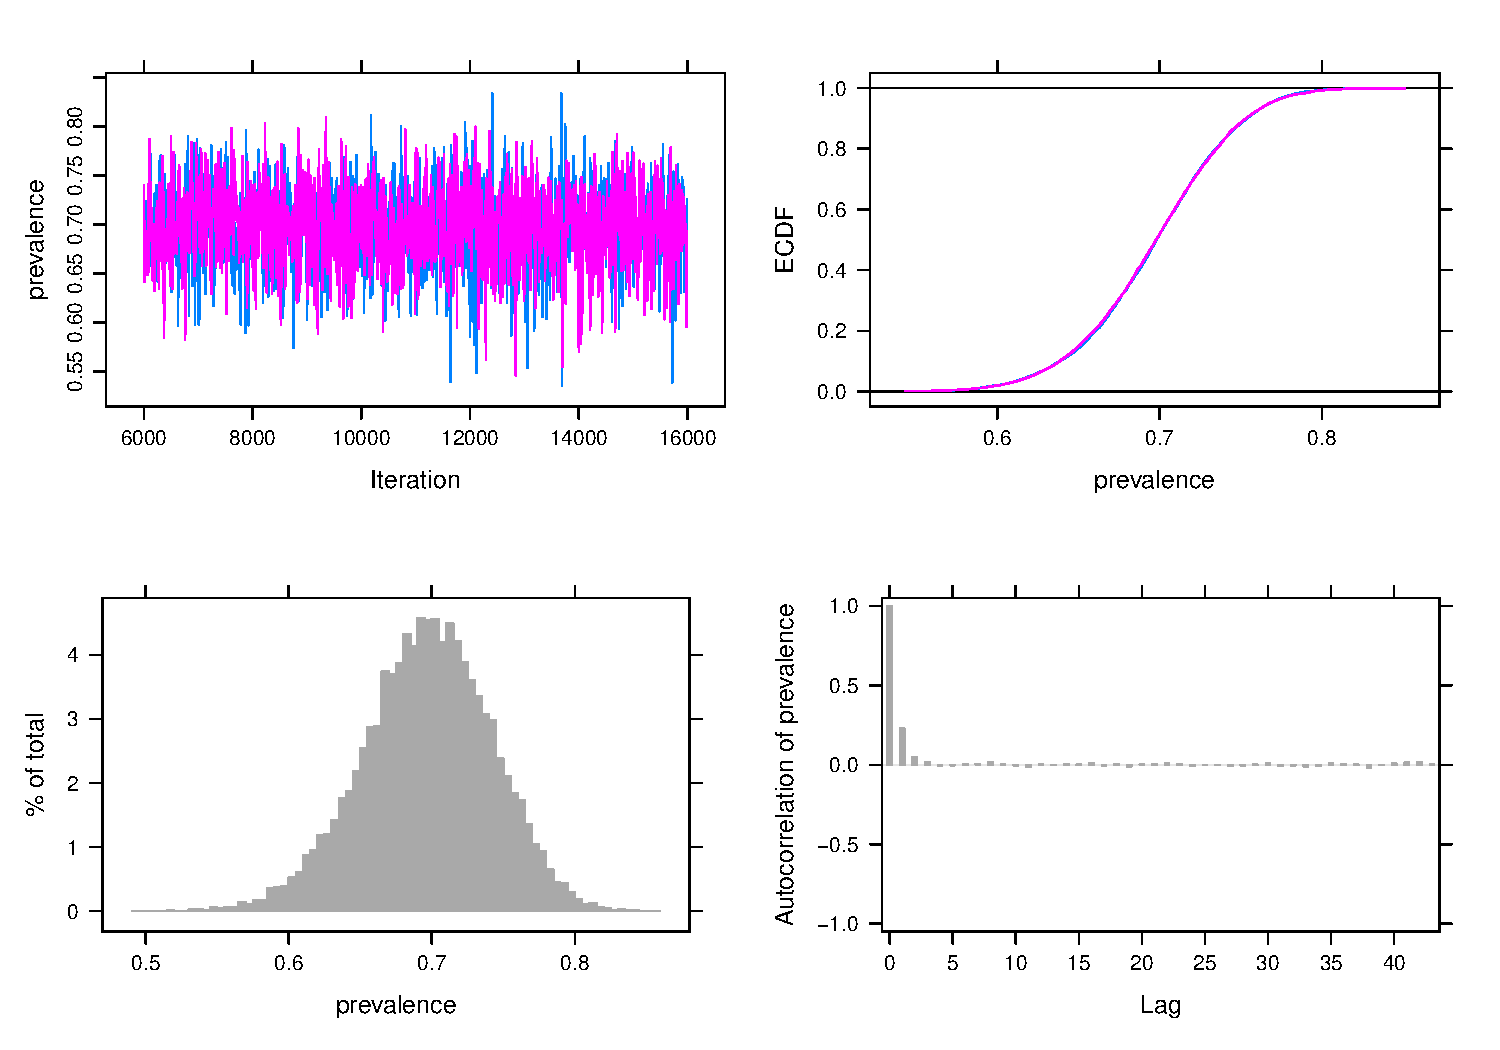
\includegraphics{Session_1_files/figure-beamer/unnamed-chunk-16-1.pdf}
\normalsize
\end{frame}

\begin{frame}
Histogram of the combined chains should appear smooth:

\scriptsize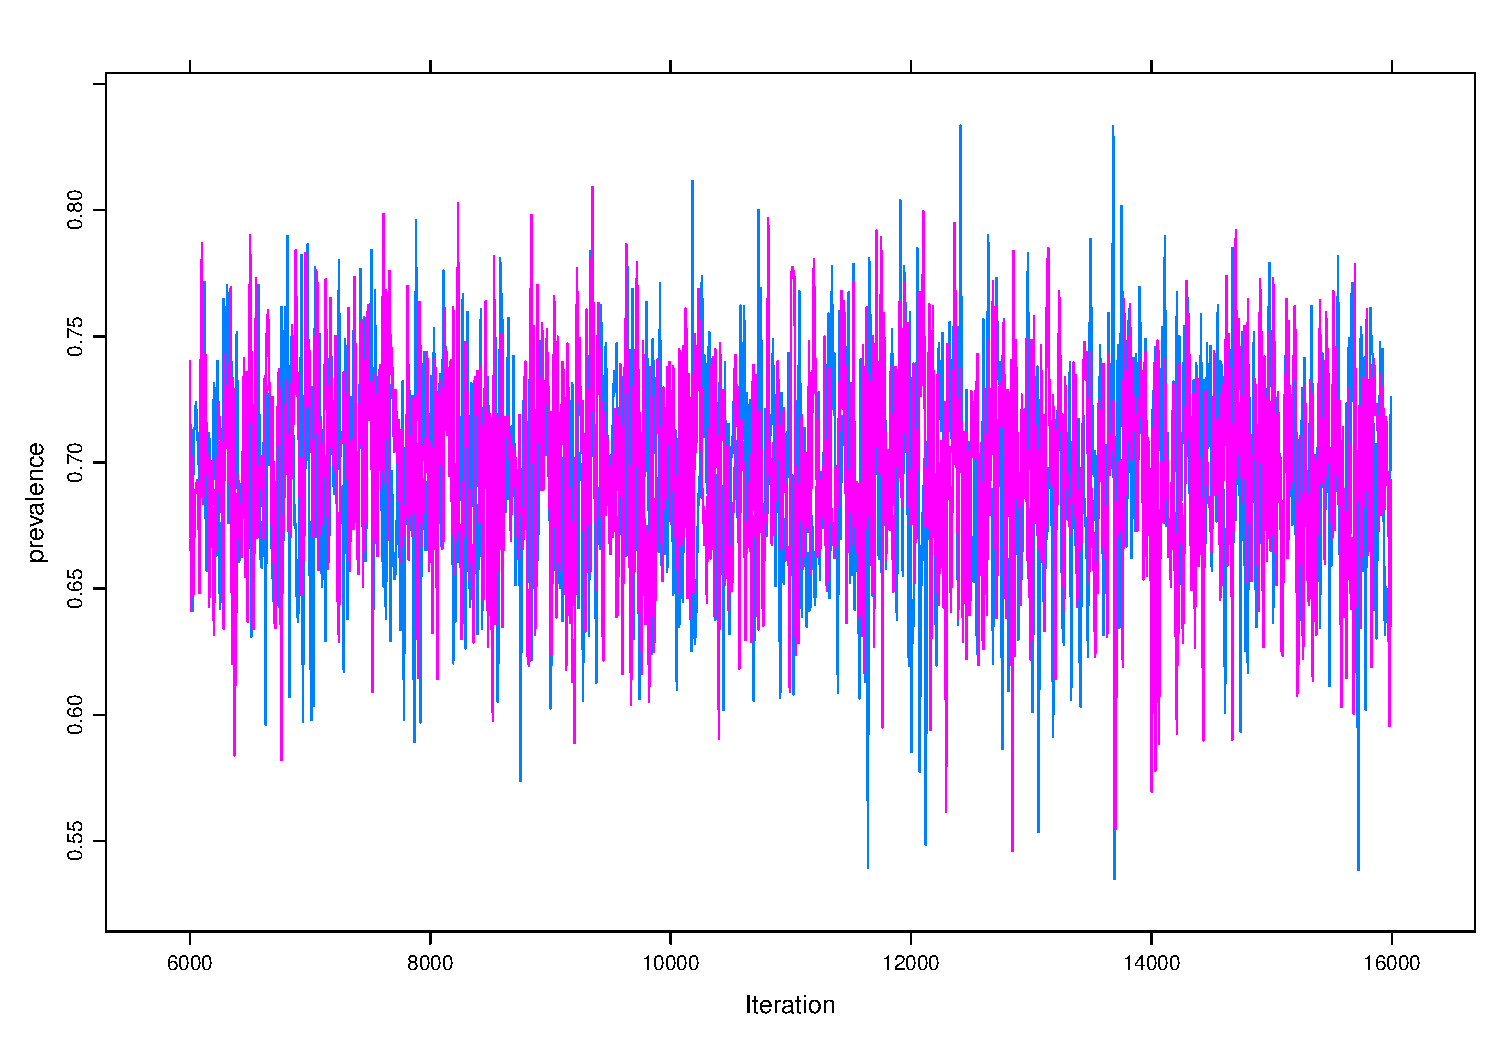
\includegraphics{Session_1_files/figure-beamer/unnamed-chunk-17-1.pdf}
\normalsize
\end{frame}

\begin{frame}
Autocorrelation plot tells you how well behaved the model is:

\scriptsize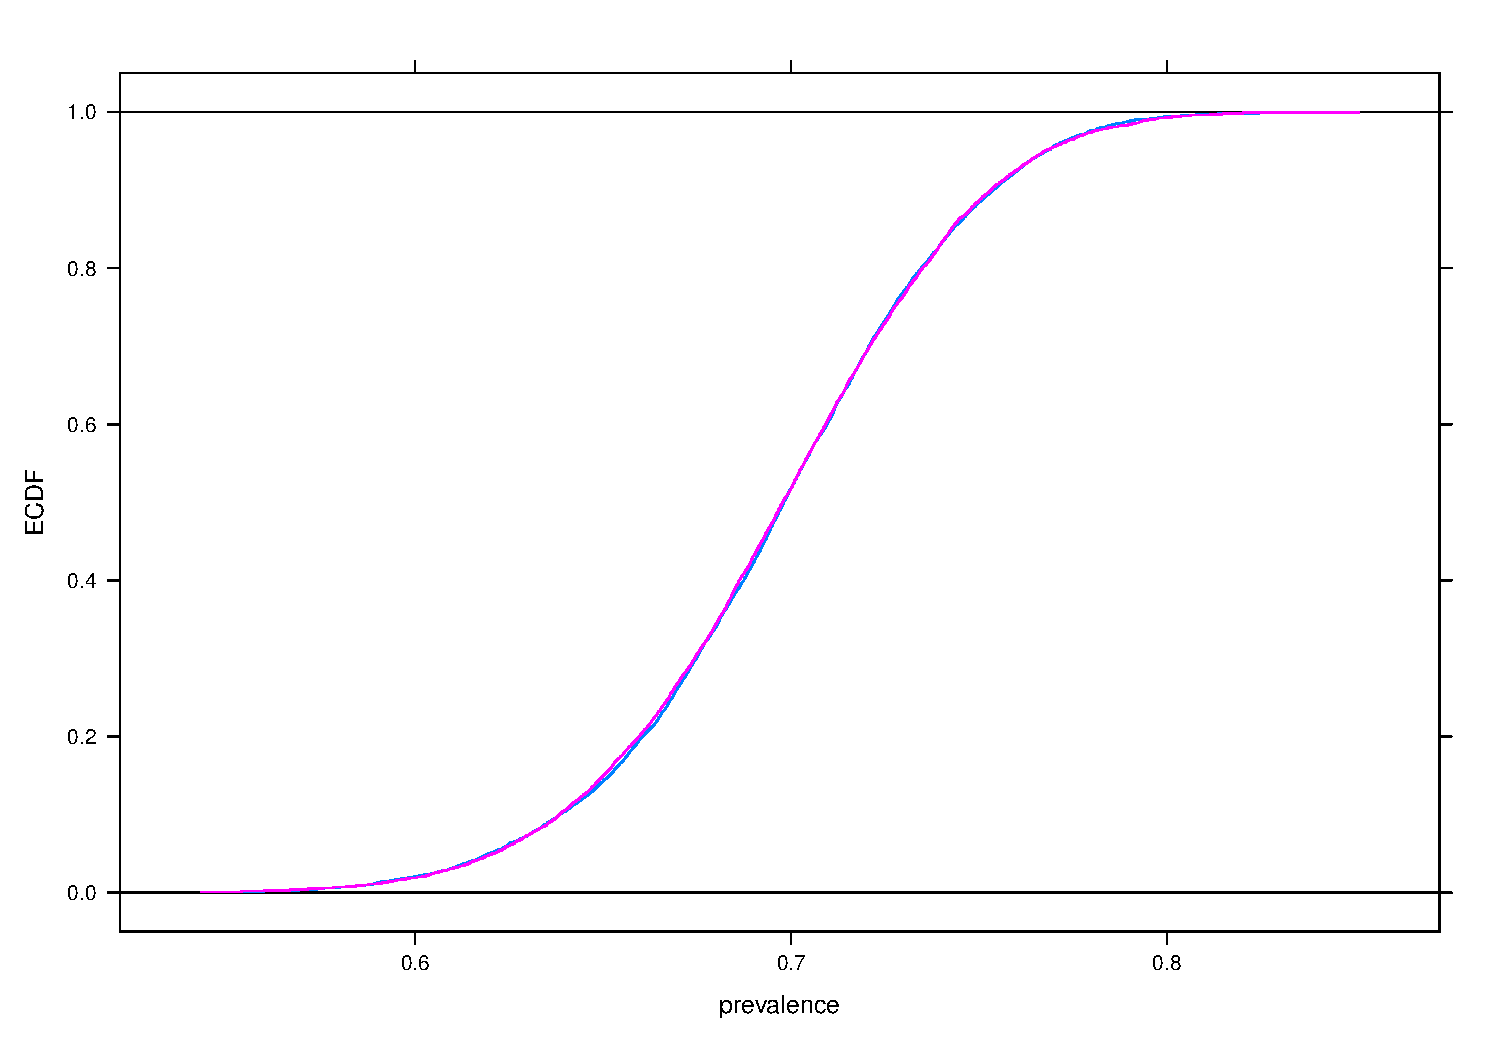
\includegraphics{Session_1_files/figure-beamer/unnamed-chunk-18-1.pdf}
\normalsize
\end{frame}

\begin{frame}[fragile]
Note: for multiple parameters, use the `back' button to cycle through
plots!

\pause

Then check the effective sample size and Gelman-Rubin statistic:

\scriptsize

\begin{Shaded}
\begin{Highlighting}[]
\NormalTok{results}
\DocumentationTok{\#\# }
\DocumentationTok{\#\# JAGS model summary statistics from 20000 samples (chains = 2; adapt+burnin = 6000):}
\DocumentationTok{\#\#                                                         }
\DocumentationTok{\#\#            Lower95  Median Upper95    Mean       SD Mode}
\DocumentationTok{\#\# prevalence 0.60905 0.69795 0.78588 0.69629 0.045261   {-}{-}}
\DocumentationTok{\#\#                                                      }
\DocumentationTok{\#\#                 MCerr MC\%ofSD SSeff     AC.10    psrf}
\DocumentationTok{\#\# prevalence 0.00040836     0.9 12285 0.0083548 0.99995}
\DocumentationTok{\#\# }
\DocumentationTok{\#\# Total time taken: 0.2 seconds}
\end{Highlighting}
\end{Shaded}

\normalsize

Reminder: we want SSeff \textgreater{} 1000 and psrf \textless{} 1.05
\end{frame}

\begin{frame}{Introduction to practical sessions}
\protect\hypertarget{introduction-to-practical-sessions}{}
Each practical session will consist of:

\begin{enumerate}
\tightlist
\item
  Some general/philosophical points to consider
\item
  One or more practical exercises to complete
\item
  One or more additional (optional) exercise for those that finish the
  main exercise early
\end{enumerate}

\pause

Consideration points are given in the PDF

The exercises (and solutions) are only in the HTML versions
\end{frame}

\begin{frame}
\begin{itemize}
\tightlist
\item
  We have approximately 30-60 mins per practical session

  \begin{itemize}
  \tightlist
  \item
    If you need help just ask!
  \item
    Otherwise we will walk around to see how you are getting on!
  \end{itemize}
\end{itemize}
\end{frame}

\hypertarget{practical-session-1}{%
\section{Practical Session 1}\label{practical-session-1}}

\begin{frame}[fragile]{Points to consider}
\protect\hypertarget{points-to-consider}{}
\begin{enumerate}
\item
  What are the advantages and disadvantages of Bayesian MCMC relative to
  more standard frequentist likelihood-based methods?
\item
  \texttt{Identifiability} refers to the ability of a model to extract
  useful information from a dataset for a particular set of parameters.
  What 3 things affect whether or not a model/parameter will be
  identifiable?
\end{enumerate}

The exercises (and solutions) can be found in Session\_1.html!

\begin{comment}

## Exercise 1 {.fragile}

Follow these steps to run the basic JAGS model given above:

- Create a new text file in RStudio by clicking on `File` then `New File` then `Text file`

- Copy the following model definition into this text file:

\scriptsize

```
model{
  # Likelihood part:
  Positives ~ dbinom(prevalence, N)
  
  # Prior part:
  prevalence ~ dbeta(1, 1)
  
  # Hooks for automatic integration with R:
  #data# Positives, N
  #monitor# prevalence
  #inits# prevalence
}
```

\normalsize

- Save the file as `basicjags.txt` in a folder where you can find it again

- Set your R working directory to the same folder, by clicking on `Session` then `Set Working Directory` then `Choose Directory` and choosing the folder location

- Create a new R file in RStudio by clicking on `File` then `New File` then `R script`, and save the file as e.g. `Session 1 exercises.R` in the same folder

- Copy and paste the following R code into this R script file:

\scriptsize

```r
library('runjags')

# data to be retrieved by runjags
Positives <- 70
N <- 100

# initial values to be retrieved by runjags:
prevalence <- list(chain1=0.05, chain2=0.95)

# run the model:
results <- run.jags('basicjags.txt', n.chains=2, burnin=5000, sample=10000)

# check convergence based on trace plots:
plot(results)

# check effective sample size and psrf, and then interpret results:
results
```

\normalsize

- Take your time to play around with this code and make sure that (1) it works, and (2) you know what is going on

- Change the initial values for prevalence to 0.5 in both chains. Does it make a difference to the output?

- Change the number of samples to e.g. 50000 or 100 - what difference does this make?

- Ask for help if you have problems!


### Solution 1 {.fragile}

The result of running your R code should look like this (where lines starting with `##` show the output of running that line of code):

\scriptsize

```r
# run the model:
results <- run.jags('basicjags.txt', n.chains=2, burnin=5000, sample=10000)

# Note: this is only commented out to save space in the exercise file!
# plot(results)

# check convergence and effective sample size, and then interpret results:
results
## 
## JAGS model summary statistics from 20000 samples (chains = 2; adapt+burnin = 6000):
##                                                         
##            Lower95  Median Upper95    Mean       SD Mode
## prevalence 0.61072 0.69836 0.78361 0.69655 0.044378   --
##                                                    
##                 MCerr MC%ofSD SSeff    AC.10   psrf
## prevalence 0.00038827     0.9 13063 0.013176 1.0003
## 
## Total time taken: 0.5 seconds
```

\normalsize

\scriptsize\normalsize

Convergence is assessed in two ways:  firstly from the trace plots, and secondly from the psrf (which is the Gelman-Rubin statistic).  The effective sample size is SSeff.  Once you are happy that the model has converged and has enough of a sample size, then you can interpret the results (typically median and 95% confidence interval estimates).

We can change the initial values like so:

\scriptsize

```r
# initial values to be retrieved by runjags:
prevalence <- list(chain1=0.5, chain2=0.5)

# run the model:
results <- run.jags('basicjags.txt', n.chains=2, burnin=5000, sample=10000)

# Note: this is only commented out to save space in the exercise file!
# plot(results)
# check convergence and effective sample size, and then interpret results:
results
## 
## JAGS model summary statistics from 20000 samples (chains = 2; adapt+burnin = 6000):
##                                                         
##            Lower95  Median Upper95    Mean       SD Mode
## prevalence  0.6073 0.69803 0.78334 0.69678 0.044989   --
##                                                       
##                 MCerr MC%ofSD SSeff       AC.10   psrf
## prevalence 0.00040086     0.9 12596 -0.00022432 1.0004
## 
## Total time taken: 0.2 seconds
```

\normalsize

This only makes a very small difference to the inference, because the model converges (and we remove burnin) in either case. The posteriors being independent of the initial values is a key assumption of using MCMC!  But remember that there will always be a small difference because MCMC is an inherently random method.  We just need to make sure that the effective sample size is high enough that this inherent randomness does not impact our inference (at least not when rounding to a sensible number of significant figures!).

Increasing the number of samples to 50000 improves the effective sample size, and therefore reduces the small random changes in the posterior inference, but also takes longer to run.  Reducing the number of samples to 100 results in an effective sample size that is too small and therefore we get unreliable estimates that change every time the model is run!

## Exercise 2 {.fragile}

We can fit the same model using frequentist maximum likelihood methods like this:

\scriptsize

```r
Positives <- 70
N <- 100

# We can time how long this takes manually:
system.time({
  # The equivalent model to JAGS:
  freq_model <- glm(cbind(Positives, N-Positives) ~ 1, family=binomial)
})
##    user  system elapsed 
##   0.003   0.000   0.004
# The intercept of the GLM is on the logit scale, so we need to take the inverse logit transform to get the prevalence:
plogis(coef(freq_model))
## (Intercept) 
##         0.7
plogis(confint(freq_model))
## Waiting for profiling to be done...
##     2.5 %    97.5 % 
## 0.6059070 0.7839748
```

\normalsize
\scriptsize\normalsize

Compare the results from the JAGS model and the frequentist model:
  - Are there any differences in the inference?
  - What about if you change the data to 7 positives out of 10?
  - Are there any practical differences between JAGS and standard GLM models?
  
Change the priors for the JAGS model from Beta(1,1) to Beta(20,1)
  - How does this affect the inference?


### Solution 2 {.fragile}

The prevalence estimate and 95% CI from the frequentist method is 0.7 (0.61 - 0.78).  The equivalent estimates from the Bayesian method are:

\scriptsize

```r
summary(results)["prevalence", c("Median","Lower95","Upper95")]
##    Median   Lower95   Upper95 
## 0.6980286 0.6073016 0.7833438
```

\normalsize

These are extremely close to each other in this case, although the same is not true with a smaller sample size:

\scriptsize

```r
Positives <- 7
N <- 10

# Frequentist analysis:
freq_model <- glm(cbind(Positives, N-Positives) ~ 1, family=binomial)
plogis(coef(freq_model))
## (Intercept) 
##         0.7
plogis(confint(freq_model))
## Waiting for profiling to be done...
##     2.5 %    97.5 % 
## 0.3934574 0.9154480
# Bayesian analysis:
results <- run.jags('basicjags.txt', n.chains=2, burnin=5000, sample=10000)

# Note: this is only commented out to save space in the exercise file!
# plot(results)
results
## 
## JAGS model summary statistics from 20000 samples (chains = 2; adapt+burnin = 6000):
##                                                        
##            Lower95  Median Upper95    Mean      SD Mode
## prevalence 0.41042 0.67728 0.90095 0.66711 0.12966   --
##                                                      
##                MCerr MC%ofSD SSeff       AC.10   psrf
## prevalence 0.0011856     0.9 11959 -0.00036431 1.0003
## 
## Total time taken: 0.1 seconds
```

\normalsize
\scriptsize\normalsize

Notice that the median estimate for the Bayesian model has shifted from 0.6980286 to 0.6772847, despite the maximum likelihood estimate remaining the same (0.7). This is due to the relatively larger impact of priors with smaller datasets.  All Bayesian models *must* include priors - even when you don't want to. We will return to this concept later today.

There is also a conceptual difference in the interpretation of the confidence intervals vs credible intervals - this is actually much easier when you are Bayesian!

The major downside of using MCMC is that it takes longer to run (glm runs in a few thousands of a second, whereas JAGS takes a few tenths of a second).  The other downside is that you have to check convergence and effective sample size manually, which is not the case for using glm().


## Exercise 3 {.fragile}

Up to now we have ignored issues of diagnostic test sensitivity and specificity.  Usually, however, we do not have a perfect test, so we do not know how many are truly positive or truly negative, rather than just testing positive or negative.  But we know that:

$$Prev_{obs} = (Prev_{true}\times Se) + ((1-Prev_{true})\times (1-Sp))$$
$$\implies Prev_{true} = \frac{Prev_{obs}-(1-Sp)}{Se-(1-Sp)}$$

[The second equation assumes that the observed prevalence and sensitivity are both higher than 1 minus the specificity!]

Using JAGS allows us to add this additional complexity to our models by including a parameter for true prevalence that is related to observed prevalence by sensitivity and specificity parameters:



\scriptsize

```
model{
  # Likelihood part:
  Positives ~ dbinom(observed_prevalence, N)
  
  # Intermediate calculations:
  observed_prevalence <- sensitivity * prevalence + (1-specificity) * (1-prevalence)
  
  # Prior part:
  sensitivity ~ dbeta(1, 1)
  specificity ~ dbeta(1, 1)
  prevalence ~ dbeta(1, 1)
  
  # Hooks for automatic integration with R:
  #data# Positives, N
  #monitor# prevalence, sensitivity, specificity, observed_prevalence
  #inits# prevalence, sensitivity, specificity
}
```

\normalsize

Copy this model to "obsprevmodel.txt" and run it yourself in JAGS.  Here is some additional R code that you will need:

\scriptsize

```r
Positives <- 70
N <- 100

# initial values to be retrieved by runjags:
prevalence <- list(chain1=0.05, chain2=0.95)
sensitivity <- list(chain1=0.95, chain2=0.05)
specificity <- list(chain1=0.05, chain2=0.95)
```

\normalsize

- Make sure that the chains have converged and that your effective sample size is sufficient. Remember that now you have multiple monitored variables, so you need to cycle through the plots using the *back* and *forward* arrows on the plot window. The very last plot is a cross-correlation plot, which shows the pairwise correlation between the estimated parameter values. What do you notice about this?

- Look at the posteriors for the 4 parameters of interest.  What do you notice about identifiability?

- Now set the sensitivity and specificity parameters to fixed values of 80% and 99% by commenting out the `sensitivity ~ dbeta(1, 1)` line and adding `sensitivity <- 0.8` in the model, and similarly commenting out the `specificity ~ dbeta(1, 1)` line and adding `specificity <- 0.99` in the model (you will also need to remove sensitivity and specificity from the #inits# line). What happens to identifiability now?


### Solution 3 {.fragile}

\scriptsize

```r
Positives <- 70
N <- 100

# initial values to be retrieved by runjags:
prevalence <- list(chain1=0.05, chain2=0.95)

# run the model:
results <- run.jags('obsprevmodel.txt', n.chains=2, burnin=5000, sample=10000)

# Note: this is only commented out to save space in the exercise file!
# plot(results)
# check convergence and effective sample size, and then interpret results:
results
## 
## JAGS model summary statistics from 20000 samples (chains = 2; adapt+burnin = 6000):
##                                                        
##                         Lower95  Median Upper95    Mean
## prevalence               0.0556 0.51811 0.99303 0.51085
## sensitivity             0.16347 0.69801 0.99974  0.6513
## specificity         0.000058295 0.31476  0.8631 0.36661
## observed_prevalence     0.60325 0.69462 0.77967 0.69335
##                                                          
##                          SD Mode      MCerr MC%ofSD SSeff
## prevalence          0.28003   --  0.0063833     2.3  1925
## sensitivity         0.22598   --  0.0058353     2.6  1500
## specificity         0.23595   --  0.0060899     2.6  1501
## observed_prevalence 0.04505   -- 0.00032226     0.7 19542
##                                      
##                          AC.10   psrf
## prevalence             0.15451 1.0024
## sensitivity            0.23169 1.0071
## specificity            0.23561 1.0042
## observed_prevalence -0.0070757 1.0002
## 
## Total time taken: 0.4 seconds
```

\normalsize

Convergence is OK and the sample size is sufficient for all parameters. The cross-correlation plot shows that the observed_prevalence parameter estimates are not correlated with those of the other parameters (green colours). However, the prevalence, sensitivity and specificity all show positive cross-correlation (yellow colours). Non-zero (i.e. either negative or positive) cross-correlation between parameters is a symptom of reduced identifiability of these parameters within the model. This is what causes the lower SSeff for these parameters relative to the observed prevalence parameter.

The posterior for `observed_prevalence` is the same as for `prevalence` in the old model.  But the posteriors for the new (true) `prevalence`, `sensitivity` and `specificity` are extremely wide!  The model is only able to identify the `observed_prevalence`, and not the other three parameters.  This is also reflected in the effective sample sizes.  There is simply not enough information to disentangle them - persuade yourself this is true by considering the following possibilities:

  - Is prevalence zero but the test is not very specific?
  - Is prevalence 100% but the test is not very sensitive?
  - Or anywhere in between?

The answer is that all are possible.  But we can make prevalence identifiable by fixing sensitivity and specificity:



\scriptsize

```
model{
  # Likelihood part:
  Positives ~ dbinom(observed_prevalence, N)
  
  # Intermediate calculations:
  observed_prevalence <- sensitivity * prevalence + (1-specificity) * (1-prevalence)
  
  # Prior part:
  #sensitivity ~ dbeta(1, 1)
  #specificity ~ dbeta(1, 1)
  sensitivity <- 0.8
  specificity <- 0.99
  prevalence ~ dbeta(1, 1)

  # Hooks for automatic integration with R:
  #data# Positives, N
  #monitor# prevalence, sensitivity, specificity, observed_prevalence
  #inits# prevalence
}
```

\normalsize

\scriptsize

```r
results <- run.jags('obsprevmodel_fixsesp.txt', n.chains=2, burnin=5000, sample=10000)
results
## 
## JAGS model summary statistics from 20000 samples (chains = 2; adapt+burnin = 6000):
##                                                            
##                     Lower95 Median Upper95    Mean       SD
## prevalence          0.75785   0.87 0.97411 0.86775 0.056203
## sensitivity             0.8    0.8     0.8     0.8        0
## specificity            0.99   0.99    0.99    0.99        0
## observed_prevalence  0.6087 0.6973 0.77954 0.69552 0.044401
##                                                  
##                     Mode      MCerr MC%ofSD SSeff
## prevalence            -- 0.00048725     0.9 13305
## sensitivity           --         --      --    --
## specificity           --         --      --    --
## observed_prevalence   -- 0.00038493     0.9 13305
##                                      
##                          AC.10   psrf
## prevalence          -0.0053803 1.0006
## sensitivity                 --     --
## specificity                 --     --
## observed_prevalence -0.0053803 1.0005
## 
## Total time taken: 0.3 seconds
```

\normalsize
Note that the true prevalence is estimated to be higher than the observed prevalence, because the test has a relatively low sensitivity.

If we don't want to fix sensitivity/specificity at specific values (which is generally a bad idea!) then we can give them a strong prior instead.  We will come back to this idea later!



## Optional Exercise A {.fragile}

- Change the number of chains to 1 and 4
  
  * Remember that you will also need to change the initial values
  * What affect does having different numbers of chains have?

- Try using the `run.jags` argument `method='parallel'` - what affect does this have?


### Solution A {.fragile}

The chains argument can be any positive integer, but you need to make sure that the number of initial values provided is consistent.  For example:

\scriptsize

```r
prevalence <- list(chain1=0.05)
sensitivity <- list(chain1=0.95)
specificity <- list(chain1=0.05)

results1 <- run.jags('obsprevmodel.txt', n.chains=1)
## Warning: Convergence cannot be assessed with only 1 chain
results1
## 
## JAGS model summary statistics from 10000 samples (adapt+burnin = 5000):
##                                                       
##                        Lower95  Median Upper95    Mean
## prevalence            0.063286 0.51719 0.99285 0.51545
## sensitivity            0.15193 0.69613 0.99997 0.64506
## specificity         0.00010507  0.3131 0.85277 0.36325
## observed_prevalence    0.60084  0.6945 0.77658 0.69345
##                                                           
##                           SD Mode      MCerr MC%ofSD SSeff
## prevalence           0.27955   --  0.0083907       3  1110
## sensitivity          0.23051   --  0.0080588     3.5   818
## specificity          0.23686   --  0.0086609     3.7   748
## observed_prevalence 0.044723   -- 0.00045768       1  9549
##                                  
##                        AC.10 psrf
## prevalence           0.15964   --
## sensitivity          0.22467   --
## specificity          0.22482   --
## observed_prevalence 0.001511   --
## 
## Total time taken: 0.3 seconds
prevalence <- list(chain1=0.05, chain2=0.4, chain3=0.6, chain4=0.95)
sensitivity <- list(chain1=0.95, chain2=0.75, chain3=0.25, chain4=0.05)
specificity <- list(chain1=0.05, chain2=0.25, chain3=0.75, chain2=0.95)
results4 <- run.jags('obsprevmodel.txt', n.chains=4)
results4
## 
## JAGS model summary statistics from 40000 samples (chains = 4; adapt+burnin = 5000):
##                                                        
##                         Lower95  Median Upper95    Mean
## prevalence             0.013047 0.50504 0.95437 0.50204
## sensitivity             0.16174 0.69294 0.99997 0.64483
## specificity         0.000042945 0.31202 0.85288 0.36337
## observed_prevalence     0.60401 0.69405 0.77909 0.69289
##                                                           
##                           SD Mode      MCerr MC%ofSD SSeff
## prevalence            0.2803   --  0.0044914     1.6  3895
## sensitivity           0.2292   --  0.0040639     1.8  3181
## specificity          0.23278   --  0.0041653     1.8  3123
## observed_prevalence 0.045066   -- 0.00022748     0.5 39247
##                                      
##                          AC.10   psrf
## prevalence             0.14979 1.0004
## sensitivity            0.21574 1.0006
## specificity            0.22726 1.0007
## observed_prevalence -0.0033586      1
## 
## Total time taken: 0.8 seconds
```

\normalsize

There are two differences:  firstly it is not possible to assess the psrf with only 1 chain (and it is harder to assess convergence generally), and secondly the effective sample size is higher with more chains as the samples are pooled (e.g. 10000 samples from 4 chains is 40000 samples).  So more chains is better.

The downside is that more chains take longer to run.  But we can offset this by parallelising:

\scriptsize

```r
results4p <- run.jags('obsprevmodel.txt', n.chains=4, method='parallel')
## Warning: You attempted to start parallel chains without
## setting different PRNG for each chain, which is not
## recommended. Different .RNG.name values have been added to
## each set of initial values.
results4p
## 
## JAGS model summary statistics from 40000 samples (chains = 4; adapt+burnin = 5000):
##                                                     
##                      Lower95  Median Upper95    Mean
## prevalence          0.045777 0.49985 0.98142 0.50214
## sensitivity           0.1482 0.69113 0.99999 0.64159
## specificity         0.000107 0.30954 0.85594 0.35965
## observed_prevalence   0.6043  0.6942  0.7822 0.69303
##                                                           
##                           SD Mode      MCerr MC%ofSD SSeff
## prevalence           0.27967   --  0.0044211     1.6  4002
## sensitivity          0.23235   --  0.0039716     1.7  3423
## specificity          0.23521   --  0.0041723     1.8  3178
## observed_prevalence 0.045297   -- 0.00023333     0.5 37686
##                                       
##                          AC.10    psrf
## prevalence             0.14613  1.0002
## sensitivity            0.21269  1.0003
## specificity            0.22754  1.0001
## observed_prevalence -0.0073249 0.99999
## 
## Total time taken: 1.3 seconds
```

\normalsize

Each chain is run in parallel, so as long as you have at least as many processors as chains then you will reduce the run time.  [Note: the run time is not reduced for this example because the model already runs very quickly and there is a small fixed overhead cost with parallelising chains, but for models that take longer to run you would see a benefit]
  
There are a large number of other options to runjags.  Some highlights:

  - The method can be parallel or background or bgparallel
  - You can use extend.jags to continue running an existing model (e.g. to increase the sample size)
  - You can use coda::as.mcmc.list to extract the underlying MCMC chains (for one more more partially matched variable name)
  - You can use the summary() method to extract summary statistics (for one more more partially matched variable name)
    * See `?summary.runjags` and `?runjagsclass` for more information

## Optional excersie B {.fragile}

There are three other ways of writing this type of model.  Using the simplest model as a template:

\scriptsize

```
model{
  # Likelihood part:
  Positives ~ dbinom(prevalence, N)
  
  # Prior part:
  prevalence ~ dbeta(1, 1)
  
  # Hooks for automatic integration with R:
  #data# Positives, N
  #monitor# prevalence
  #inits# prevalence
}
```

\normalsize

We can replace:

\scriptsize

```r
Positives ~ dbinom(prevalence, N)
```

\normalsize

with:

\scriptsize

```r
for(i in 1:N){
  Result[i] ~ dbern(prevalence)
}
```

\normalsize

or:

\scriptsize

```r
for(i in 1:N){
  NegativePositive[i] ~ dcat(observed_probabilities[1:2])
}
observed_probabilities[2] <- prevalence
observed_probabilities[1] <- 1 - prevalence
```

\normalsize

or:

\scriptsize

```r
Tally[1:2] ~ dmulti(observed_probabilities[1:2], N)

observed_probabilities[2] <- prevalence
observed_probabilities[1] <- 1 - prevalence
```

\normalsize

In each case the data is different:
- `dbern` needs the response to be a vector of 0 and 1 reflecting test results for individuals, but uses the same probability as dbinom
- `dcat` needs the response to be a vector of 1 and 2 reflecting the outcome (1=negative, 2=positive) of the test, and uses a pair of probabilities reflecting the probability of being negative and probability of being positive
- `dmulti` needs the response to be a Tally of the total number of negative tests and positive tests, and uses the same pair of probabilities as `dcat`

Try to implement these models in JAGS, and see what difference it makes to (a) the model inference, and (b) the amount of time that the model takes to run.

What are the advantages and disadvantages of each approach?

### Solution B {.fragile}

Here is the model for dbern:



\scriptsize

```
model{
  # Likelihood part:
  for(i in 1:N){
    Result[i] ~ dbern(prevalence)
  }
  
  # Prior part:
  prevalence ~ dbeta(1, 1)
  
  # Hooks for automatic integration with R:
  #data# Result, N
  #monitor# prevalence
  #inits# prevalence
}
```

\normalsize

And the necessary R code:

\scriptsize

```r
Positives <- 70
N <- 100

# initial values to be retrieved by runjags:
prevalence <- list(chain1=0.05, chain2=0.95)
sensitivity <- list(chain1=0.95, chain2=0.05)
specificity <- list(chain1=0.05, chain2=0.95)

Result <- c(rep(0, N-Positives), rep(1, Positives))
stopifnot(sum(Result)==Positives)
dbern_results <- run.jags('dbernmodel.txt', n.chains=2)
```

\normalsize

Here is the model for dcat:



\scriptsize

```
model{
  # Likelihood part:
  for(i in 1:N){
    NegativePositive[i] ~ dcat(observed_probabilities[1:2])
  }
  observed_probabilities[2] <- prevalence
  observed_probabilities[1] <- 1 - prevalence

  # Prior part:
  prevalence ~ dbeta(1, 1)
  
  # Hooks for automatic integration with R:
  #data# NegativePositive, N
  #monitor# prevalence
  #inits# prevalence
}
```

\normalsize

And the necessary R code:

\scriptsize

```r
NegativePositive <- c(rep(1, N-Positives), rep(2, Positives))
dcat_results <- run.jags('dcatmodel.txt', n.chains=2)
```

\normalsize

And here is the model for dmulti:



\scriptsize

```
model{
  # Likelihood part:
  Tally[1:2] ~ dmulti(observed_probabilities[1:2], N)

  observed_probabilities[2] <- prevalence
  observed_probabilities[1] <- 1 - prevalence
 
  # Prior part:
  prevalence ~ dbeta(1, 1)
  
  # Hooks for automatic integration with R:
  #data# Tally, N
  #monitor# prevalence
  #inits# prevalence
}
```

\normalsize

And the necessary R code:

\scriptsize

```r
Tally <- c(N-Positives, Positives)
stopifnot(sum(Tally)==N)
dmulti_results <- run.jags('dmultimodel.txt', n.chains=2)
```

\normalsize

And the results from each of them:

\scriptsize

```r
dbern_results
## 
## JAGS model summary statistics from 20000 samples (chains = 2; adapt+burnin = 5000):
##                                                        
##            Lower95  Median Upper95   Mean       SD Mode
## prevalence 0.60559 0.69736 0.78302 0.6961 0.045346   --
##                                                       
##                 MCerr MC%ofSD SSeff      AC.10    psrf
## prevalence 0.00032064     0.7 20000 -0.0019371 0.99996
## 
## Total time taken: 0.2 seconds
dcat_results
## 
## JAGS model summary statistics from 20000 samples (chains = 2; adapt+burnin = 5000):
##                                                         
##            Lower95  Median Upper95    Mean       SD Mode
## prevalence 0.60577 0.69799 0.78341 0.69612 0.045556   --
##                                                      
##                 MCerr MC%ofSD SSeff      AC.10   psrf
## prevalence 0.00041117     0.9 12276 0.00079099 1.0004
## 
## Total time taken: 0.9 seconds
dmulti_results
## 
## JAGS model summary statistics from 20000 samples (chains = 2; adapt+burnin = 5000):
##                                                         
##            Lower95  Median Upper95    Mean       SD Mode
## prevalence 0.60862 0.69786 0.78338 0.69673 0.045017   --
##                                                     
##                 MCerr MC%ofSD SSeff     AC.10   psrf
## prevalence 0.00039506     0.9 12984 0.0095339 1.0001
## 
## Total time taken: 0.2 seconds
```

\normalsize

The key points are:

  - The posteriors are the same - these are the same model just formulated differently!
  - The dcat and dbern versions take longer to run due to the loop
  - The dcat and dbern versions would allow us to fit individual-level predictors to prevalence
  - The advantage of dcat and dmulti is that we are not stuck with binary outcomes, i.e. we can have 3, 4, 5, etc different possible outcomes

You should also note that the dbern version has a higher effective sample size. The reason for this is that JAGS can use a conjugate sampler in this case; this outside the scope of this course but you can read up on what this means [here](https://en.wikipedia.org/wiki/Conjugate_prior))

If you are really interested in what kind of sampler JAGS is using for each parameter, you can always find out:

\scriptsize

```r
extract(dbern_results, "samplers")
##   Index.No             Sampler       Node
## 1        1 bugs::ConjugateBeta prevalence
extract(dcat_results, "samplers")
##   Index.No          Sampler                      Node
## 1        1 base::RealSlicer observed_probabilities[2]
extract(dmulti_results, "samplers")
##   Index.No          Sampler                      Node
## 1        1 base::RealSlicer observed_probabilities[2]
```

\normalsize

But the internal mechanisms of JAGS is well outside the scope of this course!

\end{comment}
\end{frame}

\begin{frame}[fragile]{Summary}
\protect\hypertarget{summary}{}
\begin{itemize}
\item
  MCMC allows flexibility in models BUT requires more computational
  resource and user awareness

  \begin{itemize}
  \tightlist
  \item
    Convergence
  \item
    Effective sample size
  \end{itemize}
\item
  Bayesian methods allow priors to be used BUT necessitate that priors
  are used
\item
  Models are less likely to be identifiable if they:

  \begin{itemize}
  \tightlist
  \item
    Are more complex
  \item
    Have less informative priors
  \item
    Do not have sufficient data
  \end{itemize}
\item
  There is often a disparity between the model we would like to run and
  the model we can run given the data available
\end{itemize}
\end{frame}

\end{document}
